\documentclass[11pt,a4paper]{article}

\usepackage{standalone}
\usepackage{framed}
\usepackage[dutch]{babel}
\usepackage{graphicx}
\usepackage{float}
\usepackage{csquotes}
\usepackage{color}
\usepackage{amsthm}
\usepackage{listings}
\usepackage{pdfpages}
\usepackage{amssymb}
\usepackage{graphicx}
\usepackage{caption}
\usepackage{subcaption}
\usepackage{titling}
\usepackage{amsmath}
\usepackage{textcomp}
\usepackage{multirow}
\newcommand{\subtitle}[1]{%
  \posttitle{%
    \par\end{center}
    \begin{center}\large#1\end{center}
    \vskip0.5em}%
}
\newcommand{\at}{\makeatletter @\makeatother}

\let\oldemptyset\emptyset
\let\emptyset\varnothing

\begin{document}

%%%%%%%%%%%%%%%%%%%%%%%%%%%%%%%%%%%%%%%%%
% University Assignment Title Page 
% LaTeX Template
% Version 1.0 (27/12/12)
%
% This template has been downloaded from:
% http://www.LaTeXTemplates.com
%
% Original author:
% WikiBooks (http://en.wikibooks.org/wiki/LaTeX/Title_Creation)
%
% License:
% CC BY-NC-SA 3.0 (http://creativecommons.org/licenses/by-nc-sa/3.0/)
% 
% Instructions for using this template:
% This title page is capable of being compiled as is. This is not useful for 
% including it in another document. To do this, you have two options: 
%
% 1) Copy/paste everything between \begin{document} and \end{document} 
% starting at \begin{titlepage} and paste this into another LaTeX file where you 
% want your title page.
% OR
% 2) Remove everything outside the \begin{titlepage} and \end{titlepage} and 
% move this file to the same directory as the LaTeX file you wish to add it to. 
% Then add %%%%%%%%%%%%%%%%%%%%%%%%%%%%%%%%%%%%%%%%%
% University Assignment Title Page 
% LaTeX Template
% Version 1.0 (27/12/12)
%
% This template has been downloaded from:
% http://www.LaTeXTemplates.com
%
% Original author:
% WikiBooks (http://en.wikibooks.org/wiki/LaTeX/Title_Creation)
%
% License:
% CC BY-NC-SA 3.0 (http://creativecommons.org/licenses/by-nc-sa/3.0/)
% 
% Instructions for using this template:
% This title page is capable of being compiled as is. This is not useful for 
% including it in another document. To do this, you have two options: 
%
% 1) Copy/paste everything between \begin{document} and \end{document} 
% starting at \begin{titlepage} and paste this into another LaTeX file where you 
% want your title page.
% OR
% 2) Remove everything outside the \begin{titlepage} and \end{titlepage} and 
% move this file to the same directory as the LaTeX file you wish to add it to. 
% Then add %%%%%%%%%%%%%%%%%%%%%%%%%%%%%%%%%%%%%%%%%
% University Assignment Title Page 
% LaTeX Template
% Version 1.0 (27/12/12)
%
% This template has been downloaded from:
% http://www.LaTeXTemplates.com
%
% Original author:
% WikiBooks (http://en.wikibooks.org/wiki/LaTeX/Title_Creation)
%
% License:
% CC BY-NC-SA 3.0 (http://creativecommons.org/licenses/by-nc-sa/3.0/)
% 
% Instructions for using this template:
% This title page is capable of being compiled as is. This is not useful for 
% including it in another document. To do this, you have two options: 
%
% 1) Copy/paste everything between \begin{document} and \end{document} 
% starting at \begin{titlepage} and paste this into another LaTeX file where you 
% want your title page.
% OR
% 2) Remove everything outside the \begin{titlepage} and \end{titlepage} and 
% move this file to the same directory as the LaTeX file you wish to add it to. 
% Then add \input{./title_page_1.tex} to your LaTeX file where you want your
% title page.
%
%%%%%%%%%%%%%%%%%%%%%%%%%%%%%%%%%%%%%%%%%

%----------------------------------------------------------------------------------------
%	PACKAGES AND OTHER DOCUMENT CONFIGURATIONS
%----------------------------------------------------------------------------------------

\documentclass[12pt]{article}
\newcommand{\at}{\makeatletter @\makeatother}

\begin{document}

\begin{titlepage}

\newcommand{\HRule}{\rule{\linewidth}{0.5mm}} % Defines a new command for the horizontal lines, change thickness here

\center % Center everything on the page
 
%----------------------------------------------------------------------------------------
%	HEADING SECTIONS
%----------------------------------------------------------------------------------------

\textsc{\LARGE Vrije Universiteit Brussel}\\[1.5cm] % Name of your university/college
\textsc{\Large Computersystemen:}\\[0.5cm] % Major heading such as course name
\textsc{\large "Groep 2: project Snake"}\\[0.5cm] % Minor heading such as course title

%----------------------------------------------------------------------------------------
%	TITLE SECTION
%----------------------------------------------------------------------------------------

\HRule \\[0.4cm]
{ \huge \bfseries Code verslag}\\[0.4cm] % Title of your document
\HRule \\[1.5cm]
 
%----------------------------------------------------------------------------------------
%	AUTHOR SECTION
%----------------------------------------------------------------------------------------

\begin{minipage}{0.4\textwidth}
\begin{flushleft} \large
\emph{Auteurs:}\\
J\'er\^ome \textsc{Botoko Ekila} % Your name
Arthur \textsc{Chom\'e} \\
\end{flushleft}
\end{minipage}
~
\begin{minipage}{0.4\textwidth}
\begin{flushright} \large
\emph{Richting.:} \\
Faculteit Wetenschappen
Bach. Computerwet.
\end{flushright}
\end{minipage}\\[4cm]

% If you don't want a supervisor, uncomment the two lines below and remove the section above
%\Large \emph{Author:}\\
%John \textsc{Smith}\\[3cm] % Your name

%----------------------------------------------------------------------------------------
%	DATE SECTION
%----------------------------------------------------------------------------------------

{\large \today}\\[3cm] % Date, change the \today to a set date if you want to be precise

%----------------------------------------------------------------------------------------
%	LOGO SECTION
%----------------------------------------------------------------------------------------

%\includegraphics{Logo}\\[1cm] % Include a department/university logo - this will require the graphicx package
 
%----------------------------------------------------------------------------------------

\vfill % Fill the rest of the page with whitespace

\end{titlepage}
\end{document} to your LaTeX file where you want your
% title page.
%
%%%%%%%%%%%%%%%%%%%%%%%%%%%%%%%%%%%%%%%%%

%----------------------------------------------------------------------------------------
%	PACKAGES AND OTHER DOCUMENT CONFIGURATIONS
%----------------------------------------------------------------------------------------

\documentclass[12pt]{article}
\newcommand{\at}{\makeatletter @\makeatother}

\begin{document}

\begin{titlepage}

\newcommand{\HRule}{\rule{\linewidth}{0.5mm}} % Defines a new command for the horizontal lines, change thickness here

\center % Center everything on the page
 
%----------------------------------------------------------------------------------------
%	HEADING SECTIONS
%----------------------------------------------------------------------------------------

\textsc{\LARGE Vrije Universiteit Brussel}\\[1.5cm] % Name of your university/college
\textsc{\Large Computersystemen:}\\[0.5cm] % Major heading such as course name
\textsc{\large "Groep 2: project Snake"}\\[0.5cm] % Minor heading such as course title

%----------------------------------------------------------------------------------------
%	TITLE SECTION
%----------------------------------------------------------------------------------------

\HRule \\[0.4cm]
{ \huge \bfseries Code verslag}\\[0.4cm] % Title of your document
\HRule \\[1.5cm]
 
%----------------------------------------------------------------------------------------
%	AUTHOR SECTION
%----------------------------------------------------------------------------------------

\begin{minipage}{0.4\textwidth}
\begin{flushleft} \large
\emph{Auteurs:}\\
J\'er\^ome \textsc{Botoko Ekila} % Your name
Arthur \textsc{Chom\'e} \\
\end{flushleft}
\end{minipage}
~
\begin{minipage}{0.4\textwidth}
\begin{flushright} \large
\emph{Richting.:} \\
Faculteit Wetenschappen
Bach. Computerwet.
\end{flushright}
\end{minipage}\\[4cm]

% If you don't want a supervisor, uncomment the two lines below and remove the section above
%\Large \emph{Author:}\\
%John \textsc{Smith}\\[3cm] % Your name

%----------------------------------------------------------------------------------------
%	DATE SECTION
%----------------------------------------------------------------------------------------

{\large \today}\\[3cm] % Date, change the \today to a set date if you want to be precise

%----------------------------------------------------------------------------------------
%	LOGO SECTION
%----------------------------------------------------------------------------------------

%\includegraphics{Logo}\\[1cm] % Include a department/university logo - this will require the graphicx package
 
%----------------------------------------------------------------------------------------

\vfill % Fill the rest of the page with whitespace

\end{titlepage}
\end{document} to your LaTeX file where you want your
% title page.
%
%%%%%%%%%%%%%%%%%%%%%%%%%%%%%%%%%%%%%%%%%

%----------------------------------------------------------------------------------------
%	PACKAGES AND OTHER DOCUMENT CONFIGURATIONS
%----------------------------------------------------------------------------------------

\documentclass[12pt]{article}
\newcommand{\at}{\makeatletter @\makeatother}

\begin{document}

\begin{titlepage}

\newcommand{\HRule}{\rule{\linewidth}{0.5mm}} % Defines a new command for the horizontal lines, change thickness here

\center % Center everything on the page
 
%----------------------------------------------------------------------------------------
%	HEADING SECTIONS
%----------------------------------------------------------------------------------------

\textsc{\LARGE Vrije Universiteit Brussel}\\[1.5cm] % Name of your university/college
\textsc{\Large Computersystemen:}\\[0.5cm] % Major heading such as course name
\textsc{\large "Groep 2: project Snake"}\\[0.5cm] % Minor heading such as course title

%----------------------------------------------------------------------------------------
%	TITLE SECTION
%----------------------------------------------------------------------------------------

\HRule \\[0.4cm]
{ \huge \bfseries Code verslag}\\[0.4cm] % Title of your document
\HRule \\[1.5cm]
 
%----------------------------------------------------------------------------------------
%	AUTHOR SECTION
%----------------------------------------------------------------------------------------

\begin{minipage}{0.4\textwidth}
\begin{flushleft} \large
\emph{Auteurs:}\\
J\'er\^ome \textsc{Botoko Ekila} % Your name
Arthur \textsc{Chom\'e} \\
\end{flushleft}
\end{minipage}
~
\begin{minipage}{0.4\textwidth}
\begin{flushright} \large
\emph{Richting.:} \\
Faculteit Wetenschappen
Bach. Computerwet.
\end{flushright}
\end{minipage}\\[4cm]

% If you don't want a supervisor, uncomment the two lines below and remove the section above
%\Large \emph{Author:}\\
%John \textsc{Smith}\\[3cm] % Your name

%----------------------------------------------------------------------------------------
%	DATE SECTION
%----------------------------------------------------------------------------------------

{\large \today}\\[3cm] % Date, change the \today to a set date if you want to be precise

%----------------------------------------------------------------------------------------
%	LOGO SECTION
%----------------------------------------------------------------------------------------

%\includegraphics{Logo}\\[1cm] % Include a department/university logo - this will require the graphicx package
 
%----------------------------------------------------------------------------------------

\vfill % Fill the rest of the page with whitespace

\end{titlepage}
\end{document}

\tableofcontents

\section{Inleiding}
Dit programma werd geschreven in 80386 32-bit protected mode assembly en runt in DOSBox.
Voor dit project kozen we om het klassieke arcadespel Snake na te maken. Hierbij controleert de gebruiker een slang die appels eet. Het eten van de appel resulteert in het verhogen van score. De speler verliest indien de slang zichzelf opeet. Naarmate de slang langer wordt, wordt dit moeilijker om te voorkomen.
Het eindresultaat van dit project is een werkend Snake-spel. Daarbij werden een aantal extra features toegevoegd om het spel uit te breiden.

\newpage

\section{Features}

\subsection{Start menu}

Wanneer het programma met de x86-emulator wordt gestart, verschijnt het startmenu. In dit menu heeft de gebruiker vier mogelijkheden: 
\begin{enumerate}
	\item Het spel opstarten (play game).
	\item De moeilijkheidsgraad aanpassen (difficulties).
	\item Naar de hulpsectie gaan (help) waar een kort overzicht staat van de belangrijkste spelelementen en hoe het spel te spelen.
	\item Het programma afsluiten (exit) waarbij de gebruiker terugkomt op de DOS-emulator.
\end{enumerate}
Deze opties kunnen geselecteerd worden door het pijltje links te positioneren op de gewilde actie en op 'enter' te drukken. Als alternatief om het programma af te sluiten kan de gebruiker ten alle tijde op 'escape' drukken.

\begin{figure}[h]
\centering
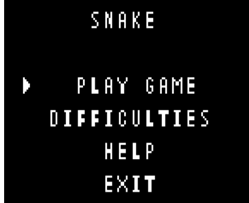
\includegraphics[scale=1]{main.png}
\caption{Kiezen in het menu}
\label{fig:menu}
\end{figure}


\subsection{Game}
Het doel van dit spel is om een zo hoog mogelijke score te behalen. Het spelscherm is eindig in omvang. Hierdoor eindigt het spel altijd door een botsing van de slang in zichzelf.

\begin{figure}[h]
\centering
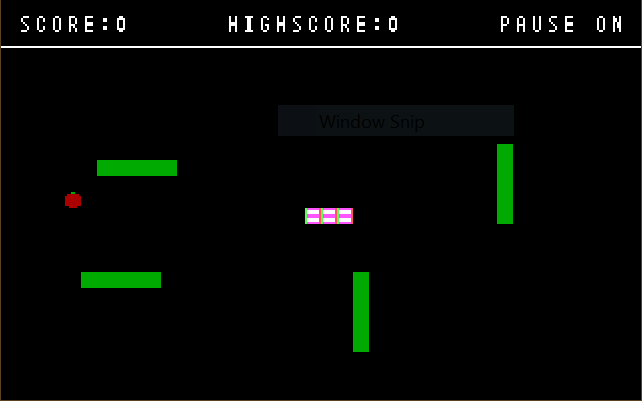
\includegraphics[scale=1]{game.png}
\caption{Het spel}
\label{fig:game}
\end{figure}

\subsubsection{Slang}
Bij de start van het spel krijgt de gebruiker direct controle van een wit-roze slang. Deze beweegt standaard naar rechts in het begin. De speler verliest indien deze zichzelf opeet of op een groene muur botst. De slang beweegt zich anders naarmate de moeilijkheid van het spel. Hoe hoger de moeilijkheid hoe sneller de slang.


\subsubsection{Appel}
Een appel verschijnt willekeurig op het scherm en verandert van locatie van tijd tot tijd. Bij het opeten van de appel wordt de slang langer. De gebruiker wordt dan ook beloont met een aantal punten voor het vangen van de appel. 

\subsubsection{Muren}
Om te voorkomen dat het spel lineair aanvoelt zonder verrassingen, worden de muren willekeurig op het spelscherm geplaatst bij elke nieuwe spelsessie. Het aantal muren die gegenereerd worden hangt af van de moeilijkheidsgraad. Zo heeft de moeilijkheid ‘baby’ geen muren, maar 'insane' een tiental.

\subsubsection{Score en highscore}
In de linkerbovenhoek zit de score. Deze kan verhoogd worden door een appel op te eten. Naarmate de moeilijkheid daalt krijgt de gebruiker meer punten voor een appel. Zo is een appel in 'baby' dubbel zoveel waard vergeleken met de moeilijkheid 'insane'. \\
Daarbij wordt de hoogst behaalde score behouden, maar deze wordt wel niet bijgehouden bij het sluiten van het spel.

\subsubsection{Pauze knop}
Door op 'p'-knop te drukken, kan de speler het spel pauzeren. Hierbij valt het spel volledig stil. De slang beweegt niet en de appel verandert niet meer van positie. 

\subsection{Moeilijkheidsgraad}
Om meer variatie in het spel te krijgen en de vaardigheden van de gebruiker te testen, beschikt de speler de keuze over zes verschillende moeilijkheden.
Het verschil tussen een lagere en hogere moeilijkheidsgraad is dat de slang sneller beweegt, het eten van een appel geeft minder punten en er worden meer muren geplaatst op het scherm.
Aan de hand van de boven en onder pijlen en 'enter' kan men dit menu navigeren en een nieuwe moeilijkheidsgraad selecteren.

\begin{figure}[h]
\centering
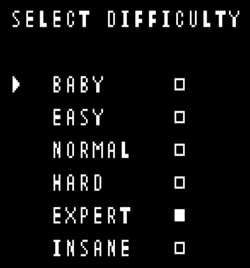
\includegraphics[scale=1]{diff.png}
\caption{Kiezen van de moeilijkheidsgraad}
\label{fig:diff}
\end{figure}

\subsection{Hulp menu}
De voorlaatste keuze in het eerste menu is de help sectie. Hier kan de gebruiker een kort overzicht vinden over de werking van het spel. Om terug naar te keren naar het eerste menu kan de gebruiker op 'escape' drukken.

\subsection{Exit}
Deze laatste optie sluit het programma volledig af. Als alternatief kan de gebruiker te allen tijde op 'escape' drukken om het programma af te sluiten.

\newpage

\section{Code}
De code is onderverdeeld in vier bestanden: game.asm, menu.asm, gui.asm en rand.asm (+ de include files). Aan de hand van de Watcom makefile kan de code gecompileerd en gelinkt worden. De resulterende executable heet 'snake.exe'.

\subsection{Menu}
De start van het programma bevindt zich in 'menu.asm'. Dit bestand omvat 'game' en 'gui' met de nodige includes. Bij de start wordt de VGA kaart geschakeld naar modus 13h om het tekenen van pixels toe te laten.\\
We hebben twee verschillende input handlers voor de twee eerste opties. De loop van 'help' is feitelijk de input handler zelf: wachten op 'escape'. Ten laatste draait het programma volledig in het spel gedeelte indien game aangeroepen is. De functie 'runGame' is namelijk een loop die enkel zal terugkeren naar het menu bij het oproepen van exit in 'game.asm'.

\subsection{Game}
Voordat men in de interne loops terechtkomt, worden alle spelvariabelen eerst geïnitialiseerd door 'initGameState'. Het centraliseren van deze variabelen betekent dat het eenvoudig is om ze snel aan te passen.

In de loop van het spel wordt de interactie procedure aangeroepen en mogelijks op gereageerd (bijvoorbeeld het aanpassen van de volgende richting van de slang). Hierna wordt het spel bevordert met het oproepen van 'updateGame'. Het spel daarentegen wordt echter enkel echt gevordert om de zoveel iteraties. Dit bepaalt de snelheid van het spel (en vervolgens de moeilijkheidsgraad) en kan gecontroleerd worden aan de hand van de variabele 'GAME\_COUNTER\_MAX'. Hierna wordt het spel scherm opnieuw getekend. 

Indien de interactie procedure vaststelt dat de 'escape' knop is ingedrukt, keert het programma in de volgende loop terug naar het menu.

\subsection{Apple generator}
De appel verandert van tijd tot tijd naar een andere willekeurige positie. De procedures die dit afhandelen zijn 'placeRandomApple' en 'drawApple'.
'placeRandomApple' gaat een nieuwe positie berekenen voor de appel en de counter resetten. Deze laatst houdt bij hou lang een appel al op dezelfde positie staat. Het bereken van een nieuwe positie gebeurt door twee keer de procedure 'rand' op te roepen: de eerste keer voor de x-co\"ordinaat en de tweede keer voor de y-co\"ordinaat. Rand steekt in register 'eax' een 32 bit getal. Dit getal delen we door de breedte (of hoogte) van het scherm. Het resultaat is de rest van de deling (modulo) en een getal tussen 0 en de breedte van het scherm. Deze co\"ordinaten moeten zich niet in een stuk van de slang of een muur bevinden. Dit is mogelijk door de positie van een appel steeds te vergelijken met elk stuk slang in 'SNAKE\_X(/Y)'. Hierbij vermenigvuldigen we de index (ten opzichte van het adres van de kop op positie 0) met 4 bytes aangezien we te werk gaan met double words.

\subsection{Wall generator}
Muren worden willekeurig gegenereerd met de procedure 'generateWalls' en onderverdeeld in muur segmenten van een bepaalde lengte. 
De eerste stap in het algoritme is het aanmaken van random x -en y-co\"ordinaten door gebruik te maken van de procedure 'rand' zoals beschreven in het vorige deel. \\
De richting (verticaal of horizontaal) van het segment wordt bij elk nieuw segment gealterneerd.

\subsection{GUI}
De slang wordt voorgesteld in twee variabelen: 'SNAKE\_X' en 'SNAKE\_Y'. Beide zijn onge\"initialiseerd gealloceerd in het geheugen. Tupels op dezelfde index van deze twee vormen een stukje van de slang. Het hoofd van de slang is het eerste tupel. Het aantal vereiste tupels is gelijk aan het aantal mogelijke ‘tiles’ op het spelbord. Dit bedraagt namelijk 1000 (40*25) double words voor beide assen. Hetzelfde principe geldt voor de muren. De grootte van een tile (op de 'grid') wordt gedefinieerd door de GUI. \\
Op deze manier staat de game los van de GUI. Het spel geeft aan wat er moet getekend worden en geeft 'grid' posities door. De GUI berekent hierna welke pixels in de videobuffer getekend moeten worden. 

\subsubsection{Wat tekenen?}
Om te beginnen kozen we om enkel veranderingen te tekenen op het bord.
Dit in tegenstelling tot het bijhouden van wat er zich in elke grid-positie bevindt.
Een voorbeeld hiervan is het bewegen van de slang. Eerst tekenen we de staart van de slang weg (kan gemakkelijk berekent worden aan de hand van de variabele 'SNAKE\_LENGTH'). Daarna tekenen we een nieuw hoofd op de volgende positie. Natuurlijk moeten we dan wel alle tupels updaten met hun volgende positie. Deze volgende positie is dan het data-element in de vorige 4 bytes (aangezien elk data element 4 bytes groot is) in beide 'SNAKE\_X' en 'SNAKE\_Y'.

\subsubsection{Tekenen van berichten}
We kwamen tot de conclusie dat het deconstrueren van een string door elke letter af te gaan en vergelijken niet zo effici\"ent verliep. Het tekenen van bijvoorbeeld 'zzz' neemt bijvoorbeeld $26*3$ vergelijkingen (voor elke letter van het alfabet) om te voltooien.
Behalve de getallen van de score waren alle andere strings in elke iteratie van het spel steeds hetzelfde. Daarom kozen we om de volgorde van sprites te defini\"eren in het data segment. Op deze manier kunnen we starten met een pointer naar het eerste data element (de eerste letter) en hierop verder dan itereren.

\section{Afhankelijkheidsdiagram}
Dit afhankelijkheidsdiagram geeft een geheeld beeld over de design van het programma.

\begin{figure}[h]
\centering
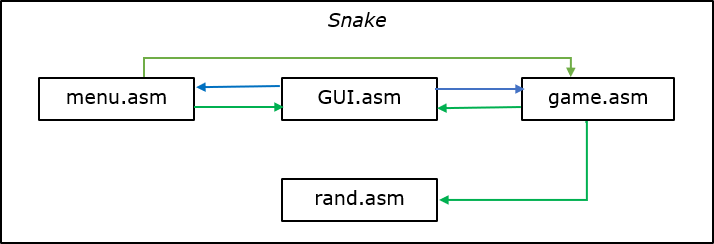
\includegraphics[scale=1]{afhank.png}
\caption{Code design SNAKE}
\label{fig:afhankelijkhedendiagram}
\end{figure}

\begin{figure}[h]
\centering
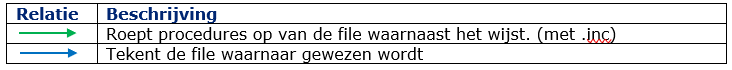
\includegraphics[scale=1]{relat.png}
\label{fig:relations}
\end{figure}

\end{document}